
\newcommand{\Integral}[2]{solutions/2017/june/118/figures/\ensuremath{\int\limits_{#1}^{#2}}}
For the random variable $X$, the CDF is
\begin{align}
    F(x)&=\Integral{0}{x}f(y)dy\\
        &=\Integral{0}{\mu}0 dy +\Integral{\mu}{x}\alpha\brak{y-\mu}^{\alpha -1}e^{-\brak{y-\mu}^\alpha}\\
        &=0 -e^{-\brak{y-\mu}^\alpha}\Big|_{\mu}^{x}\\
        &=1-e^{-\brak{x-\mu}^{\alpha}}
\end{align}
For X, the hazard function $H(y)$ is defined as
\begin{align}
    H(y)&=\frac{f(y)}{1-F(y)}\nonumber\\
    \implies H(y)&=\begin{cases}\frac{\alpha\brak{y-\mu}^{\alpha -1}e^{-\brak{y-\mu}^\alpha}}{1-\brak{1-e^{-\brak{y-\mu}^{\alpha}}}};&y>\mu\\
                        0                               &y\leq\mu   
    \end{cases}\nonumber\\
    &=\begin{cases}\alpha\brak{y-\mu}^{\alpha -1};&y>\mu\\
                        0                            &y\leq\mu   
    \end{cases}\nonumber
\end{align}
Differentiating $H(y)$ w.r.t. $y$
\begin{align}
    H'(y)&=\begin{cases}\alpha\brak{\alpha - 1}\brak{y-\mu}^{\alpha -2};&y>\mu\\
                        0                            &y\leq\mu   
    \end{cases}\nonumber
\end{align}
When $y\leq \mu$ then $H'(y)$ is $0$. When $y>\mu$ then $\brak{y-\mu}^{\alpha -2}$ is positive. This implies that the sign for $H'(y)$ for $y>\mu$ is decided by the sign of $\alpha\brak{\alpha -1}$.
\begin{align}
    \alpha\brak{1-\alpha}<0
    \implies 0<\alpha<1\nonumber\\
    \alpha\brak{1-\alpha}>0\implies \alpha>1 &&\text{(ignoring $\alpha<0$)}\nonumber
\end{align}
$\therefore$ The Hazard function of $X$ is decreasing when $\alpha \in \brak{0,1}$ and increasing when $\alpha \in \brak{1,\infty}$
\vspace{0.5cm}\centering \boxed{\solution{\text{Options 3, 4}}}
% \iffalse
% \begin{figure}[h!]
%     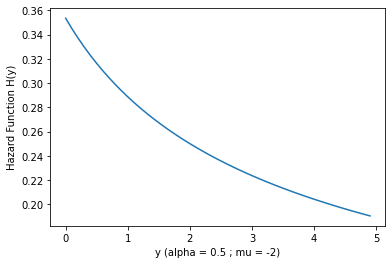
\includegraphics[width = \columnwidth]{solutions/2017/june/118/figures/Figure-1.png}
%     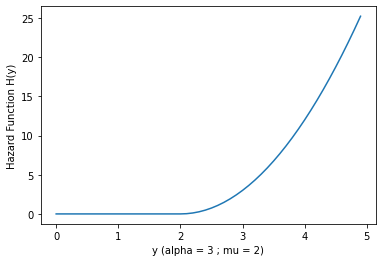
\includegraphics[width = \columnwidth]{solutions/2017/june/118/figures/Figure-2.png}
% \end{figure}
% \fi
\begin{figure}[h]
    \centering
    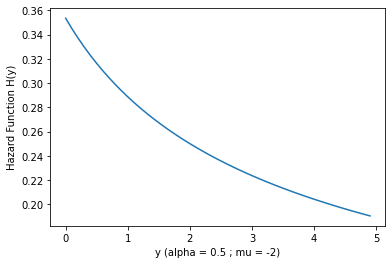
\includegraphics[width=\columnwidth-50pt]{solutions/2017/june/118/figures/Figure-1.png}
    \caption{Decreasing Hazard Function}
    \label{june/2017/118/fig:my_label1}
\end{figure}
\begin{figure}[h]
    \centering
    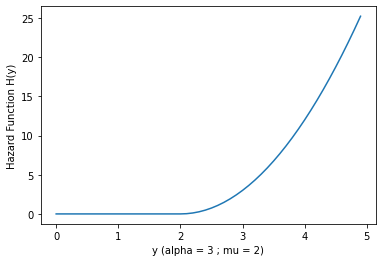
\includegraphics[width=\columnwidth-50pt]{solutions/2017/june/118/figures/Figure-2.png}
    \caption{Increasing Hazard Function}
    \label{june/2017/118/fig:my_label2}
\end{figure}
